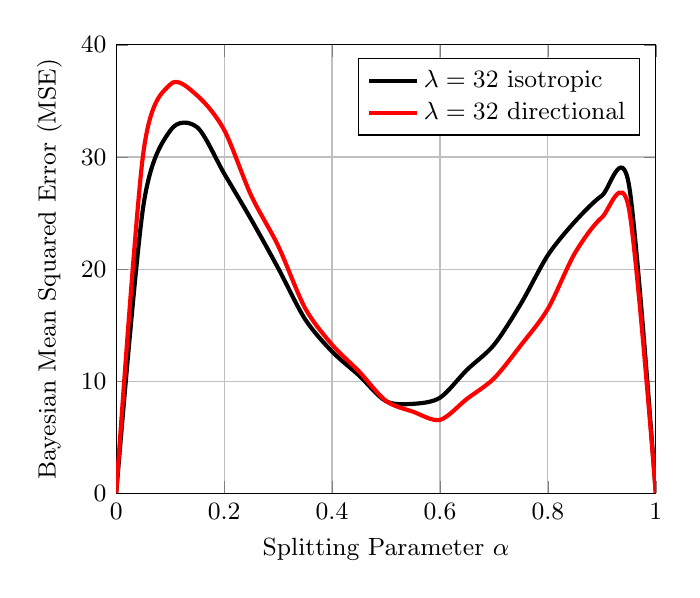
\begin{tikzpicture}
\begin{axis}[
font=\small,
xlabel= {Splitting Parameter $\alpha$},
ylabel= {Bayesian Mean Squared Error (MSE)},
xmin = 0, xmax = 1,
ymin = 0, ymax = 40,
xmajorgrids,
ymajorgrids,
legend entries={$\lambda=32$ isotropic,$\lambda=32$ directional},
legend style={legend pos=north east,nodes=right}]

% Method: Bayes,
% Area Type = inscribed,
% Antenna Type = omnidirectional,
% Noise = 2,
% Trials = 50000,
% Total rate = 16,
% alpha_step =0.025,
% A_t =36.0,
% A_o =64.0,
% BMSE

\addplot [
color=black,
line width=1.5pt,
solid,smooth,
]
coordinates{
(0.0, 0)
(0.05, 25.521)
(0.1, 32.345)
(0.15, 32.654)
(0.2, 28.532)
(0.25, 24.442)
(0.3, 20.098)
(0.35, 15.533)
(0.4, 12.641)
(0.45, 10.509)
(0.5, 8.21)
(0.55, 7.976)
(0.6, 8.521)
(0.65, 11.011)
(0.7, 13.233)
(0.75, 16.912)
(0.8, 21.243)
(0.85, 24.232)
(0.9, 26.552)
(0.95, 27.567)
(1.0, 0)
};

% Method: Bayes,
% Area Type = inscribed,
% Antenna Type = directional,
% Noise = 2,
% Trials = 50000,
% Total rate = 16,
% alpha_step =0.025,
% A_t =36.0,
% A_o =64.0,
% BMSE


\addplot [
color=red,
line width=1.5pt,
solid,smooth,
]
coordinates{
	(0.0, 0)
	(0.05, 30.254)
	(0.1, 36.466)
	(0.15, 35.488)
	(0.2, 32.421)
	(0.25, 26.574)
	(0.3, 22.087)
	(0.35, 16.523)
	(0.4, 13.254)
	(0.45, 10.866)
	(0.5, 8.233)
	(0.55, 7.275)
	(0.6, 6.543)
	(0.65, 8.421)
	(0.7, 10.241)
	(0.75, 13.211)
	(0.8, 16.457)
	(0.85, 21.423)
	(0.9, 24.609)
	(0.95, 25.425)
	(1.0, 0)
};

\end{axis}

\end{tikzpicture}

